\documentclass[border=0.125cm]{standalone}
\usepackage{tikz}
\usepackage{pgfplots}
\usepackage{graphicx}

\usetikzlibrary{decorations.pathmorphing}
\pgfplotsset{compat=newest}
\usetikzlibrary{shapes.geometric,arrows,fit,matrix,positioning}
\tikzset{main node/.style={circle,fill=black!20,draw,minimum size=3.5mm,inner sep=0pt},
         every node/.style={circle,fill=black,draw,minimum size=1mm,inner sep=0pt,label distance=-1mm},
         subtree/.style={isosceles triangle,fill=black!20,draw,minimum size=6mm,inner sep=0pt,shape border rotate=90},
         edge label/.style = {rectangle,draw=none,fill=none}
}
\begin{document}
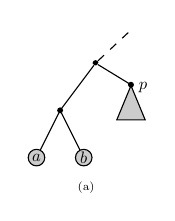
\begin{tikzpicture}[-,>=stealth', 
level 1/.style={sibling distance = 15mm},
level distance = 0.7cm, 
scale=0.6,
transform shape]

\node[edge label] {}
child[dashed]{
    [level distance = 1cm]node (0) {}
        child[solid]{
            [sibling distance = 10mm] node (1) {}
                child{
                    node [main node] (2) {$a$}
                }
                child{
                    node [main node] (3) {$b$}
                }
        }
        child[solid,edge from parent path = {(\tikzparentnode) -- (\tikzchildnode.north)}]{
            node [subtree] (4) {}
        }
}
child[missing]{node {}}
;
\node at (4.north) {};
\node[edge label,above right = 2mm and 0 mm of 4] {$p$};
\node [edge label, xshift = -2mm, below=25mm, align=flush center] at (0){
        \scriptsize{(a)}}; 
\end{tikzpicture}
~~~~~
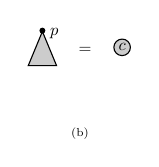
\begin{tikzpicture}[-,>=stealth', 
level 1/.style={sibling distance = 20mm},
level distance = 0.7cm, 
scale=0.6,
transform shape]

\node [subtree] (p) {};
\node at (p.north) {};
\node[edge label,above right = 2mm and 0 mm of p] {$p$};
\node [main node,above right = -1mm and 14mm of p] {$c$};
\node[edge label,above right = -1mm and 6mm of p] {$=$};

\node [edge label, below right = 15mm and 6mm of p, align=flush center] at (p){
        \scriptsize{(b)}}; 
\end{tikzpicture}
~~~~~
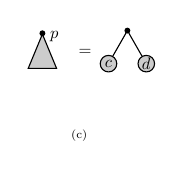
\begin{tikzpicture}[-,>=stealth', 
level 1/.style={sibling distance = 8mm},
level distance = 0.7cm, 
scale=0.6,
transform shape]
\node[edge label] at (0,-1.15){};
\node [subtree] (p) {};
\node at (p.north) {};
\node[edge label,above right = 2mm and 0 mm of p] {$p$};
\node[above right = 4mm and 16mm of p] {}
    child{node [main node] {$c$}}
    child{node [main node] {$d$}}
;
\node[edge label,above right = -1mm and 6mm of p] {$=$};
\node [edge label, below right = 15mm and 6mm of p, align=flush center] at (p){
        \scriptsize{(c)}}; 
\end{tikzpicture}

\end{document}






